\chapter{Tasks}


\section{Train Subsystem}


\begin{figure}[h]
	\centering
	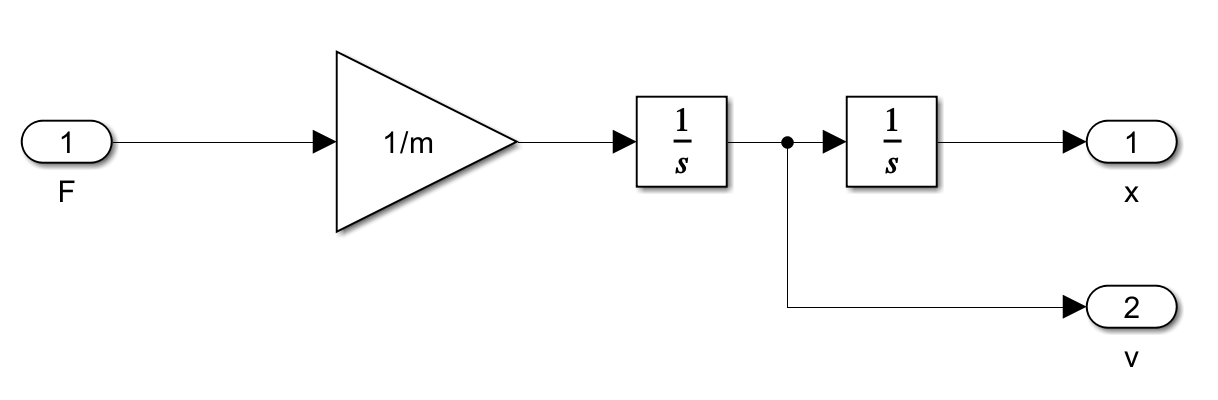
\includegraphics[width=0.8\linewidth]{images/train_subsystem.png}
	\caption{Train Subsystem}
	\label{tss}
\end{figure}

Figure \ref{tss} shows a simulink subsystem that models a train with one input, the accelerating force and two outputs, one being the distance traveled and the other the current speed.
The incoming force is converted into the acceleration according to the equation $F = m\cdot a$ by dividing by the mass, which is then turned into the velocity and distance by using two integrating blocks.

\section{Simulink Model}


The whole Simulink Model with the control loop can be seen in Figure \ref{sm}. It contains the standard control loop with a fuzzy controller and the train model mentioned above. The fuzzy controller has both the control deviation of the distance and the current speed as input signals. With the step function as target value, a distance to be traveled is specified.



\newpage
\begin{figure}[h]
	\centering
	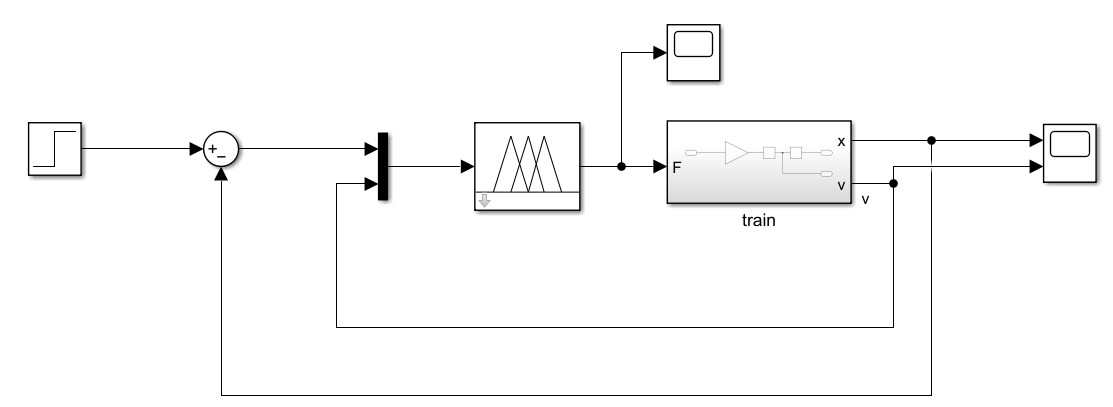
\includegraphics[width=1\linewidth]{images/simulink_model.png}
	\caption{Simulink Model}
	\label{sm}
\end{figure}


\section{Fuzzy Inference System}

The Fuzzy Inference System matrix of the Fuzzy controller can be easily edited using the Matlab Fuzzy Logic Designer. The inputs \glqq deltaX\grqq{} and \glqq v\grqq{} as well as the output \glqq F\grqq{} are implemented according to the following Membership function plots:

\begin{figure}[h]
	\centering
	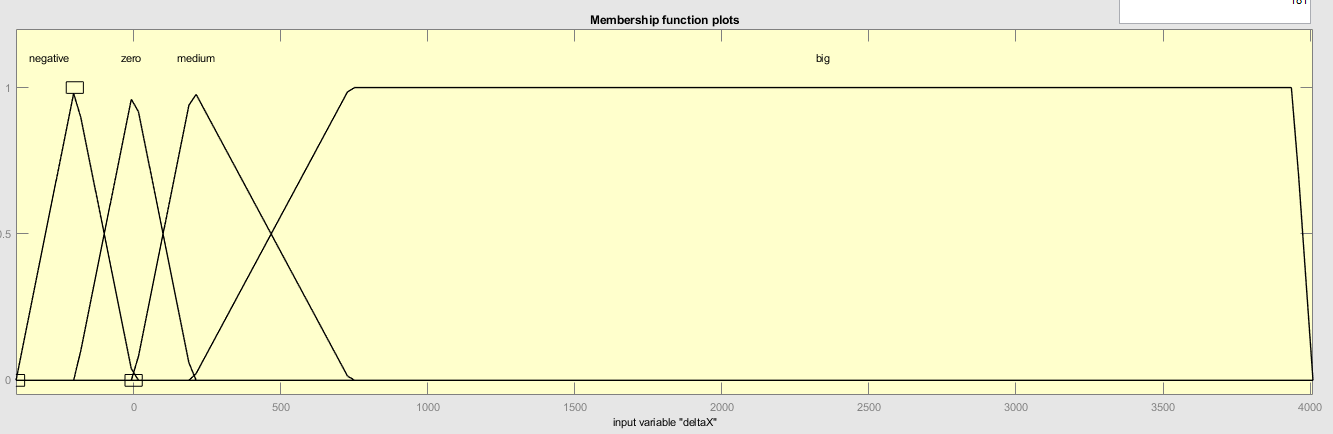
\includegraphics[scale=0.35]{images/mfp_deltax.png}
	\caption{Membership Function Plots of \glqq deltaX\grqq{}}
	\label{lolo}
\end{figure}


\begin{figure}[h]
	\centering
	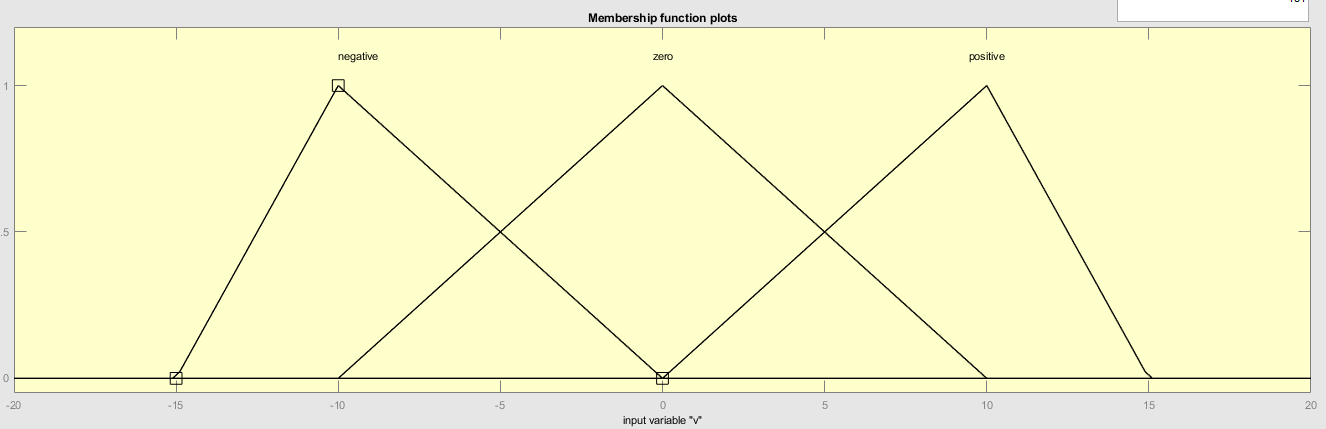
\includegraphics[scale=0.35]{images/mfp_v.png}
	\caption{Membership Function Plots of \glqq v\grqq{}}
	\label{lele}
\end{figure}


\newpage

\begin{figure}[h]
	\centering
	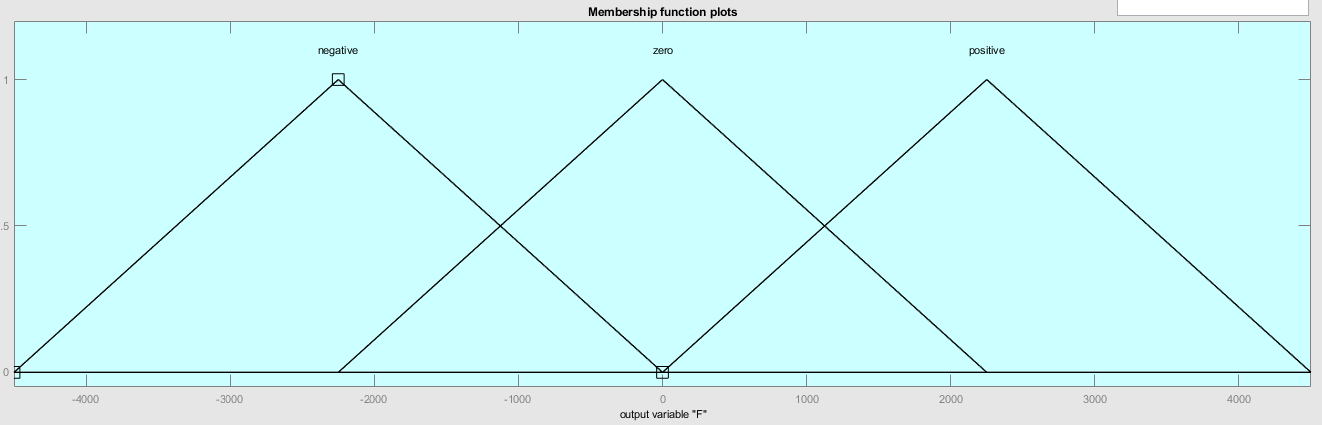
\includegraphics[scale=0.35]{images/mfp_F.png}
	\caption{Membership Function Plots of \glqq F\grqq{}}
	\label{}
\end{figure}



The Output F is calculated according to the Fuzzy rule table in Figure \ref{rules}


\begin{figure}[h]
	\centering
	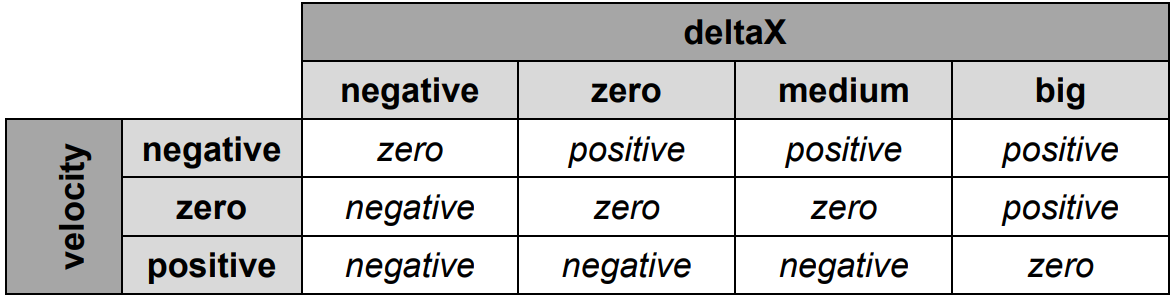
\includegraphics[width=0.9\linewidth]{images/rule_table.png}
	\caption{Fuzzy Rule Table}
	\label{rules}
\end{figure}


\section{Possible Membership Function Shapes}

The following shapes of Membership Functions are possible in the Matlab Membership Function Editor:

\begin{itemize}
	\item \texttt{trimf}: Triangular
	\item \texttt{trapmf}: Trapezoidal
	\item \texttt{gbellmf}: Generalized Bell
	\item \texttt{gaussmf}: Gaussian
	\item \texttt{gauss2mf}: Generalized Gaussian
	\item \texttt{sigmf}: Sigmoidal
	\item \texttt{dsigmf}: Difference of Sigmoids
	\item \texttt{psigmf}: Product of Sigmoids
	\item \texttt{pimf}: Pi-Shaped
	\item \texttt{smf}: S-Shaped
	\item \texttt{zmf}: Z-Shaped
	\item \texttt{linsmf}: Linear S-Shaped
	\item \texttt{linzmf}: Linear Z-Shaped
\end{itemize}



\section{Simulation}

The simulation results for a simulation time of 500 s and a distance of 2 km can be seen in figure \ref{x} for the position of the train and in figure \ref{v} for the velocity of the train. The train reaches the second station after approximately 350 seconds.

\begin{figure}[h]
	\centering
	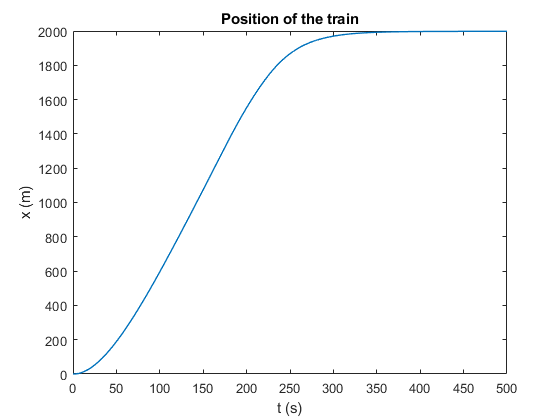
\includegraphics[width=0.9\linewidth]{images/position.png}
	\caption{Position Plot after Simulation}
	\label{x}
\end{figure}
\newpage



\begin{figure}[h]
	\centering
	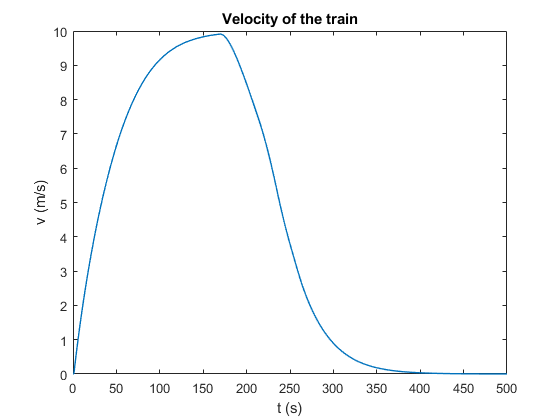
\includegraphics[width=0.9\linewidth]{images/velocity.png}
	\caption{Velocity Plot after Simulation}
	\label{v}
\end{figure}


\section{Rule Viewer}

The reason for a maximum speed of 10 $\frac{m}{s}$ or 36 $\frac{km}{h}$ is apparent from Figures \ref{lele} and \ref{rules}. From a speed of 10 $\frac{m}{s}$, $\mu_{zero} = 0$ and $\mu_{positive} = 1$, which in turn means that only the last line of the rule table is relevant, where only \glqq zero\grqq{} or \glqq negative\grqq{} are possible as output values for the force, meaning the velocity cannot rise any further.
\\
\\
The train is able to handle distances between the two stations as long as these values are defined in the membership functions for deltaX. If the distance is no longer less than 4010 m (maximum value to be defined in figure \ref{lolo}), then no membership function of deltaX is $\neq 0$, none of the rules are fulfilled and no output value can be calculated for the accelerating force.





